\documentclass[11pt,a4paper]{article}
\usepackage{ctex}
\usepackage{graphicx}
\usepackage{amsmath}
\usepackage{caption}
\usepackage{subcaption}
\usepackage{geometry}
\geometry{margin=1in}
\title{泊松图像融合实验报告}
\author{21 刘行}
\date{\today}

\begin{document}

\maketitle

	\section{实验原理}
		\subsection{PDE 构造}
			泊松图像融合 (Poisson Image Editing) 通过求解带边界条件的泊松方程, 实现源图像区域无缝粘贴到目标图像上. 基本思想是: 目标区域内部的像素值应尽量保持源图像的梯度场, 同时与边界区域保持一致, 从而达到自然融合效果.

			设目标图像为 $I_d$, 源图像为 $I_s$, 融合区域为 $\Omega$, 边界为 $\partial\Omega$. 我们的目标是求解如下偏微分方程:
			\begin{equation*}
				\min_{f} \int_\Omega \|\nabla f - \mathbf{v}\|^2 \quad \text{subject to} \quad f|_{\partial\Omega} = f^*|_{\partial\Omega}
			\end{equation*}

			其中 $\mathbf{v} = \nabla I_s$ 表示源图像在融合区域的梯度场, $f^*$ 是目标图像. 令 $E(f) = \int_\Omega \|\nabla f - \mathbf{v}\|^2\,\text{d}x$, 取变分 $\delta E = 0$, 得:
			\begin{equation*}
				\delta E = \int_\Omega 2(\nabla f - \mathbf{v}) \cdot \nabla \delta f\,\text{d}x = -2\int_\Omega \operatorname{div}(\nabla f - \mathbf{v}) \delta f\,\text{d}x \Rightarrow \Delta f = \operatorname{div}(\mathbf{v})
			\end{equation*}

			于是该变分问题等价于求解以下泊松方程:
			\begin{equation*}
				\Delta f = \text{div}(\mathbf{v}) \quad \text{in } \Omega, \quad f|_{\partial\Omega} = f^*|_{\partial\Omega}
			\end{equation*}

		\subsection{矩阵构造与求解}
			对融合区域内的每个像素, 建立五点差分离散方程:
			\begin{equation*}
				4f_{i,j} - f_{i+1,j} - f_{i-1,j} - f_{i,j+1} - f_{i,j-1} = \text{div}(\mathbf{v})_{i,j}
			\end{equation*}

			如果混合梯度启用, 我们对源图和目标图的梯度分别计算并选取绝对值更大的项:
			\begin{equation*}
				\mathbf{v}_{i,j} =
				\begin{cases}
					\nabla I_s & \text{if } |\nabla I_s| > |\nabla I_d| \\
					\nabla I_d & \text{otherwise}
				\end{cases}
			\end{equation*}

			矩阵 $A$ 为稀疏对称正定, 其大小为 $N \times N$, 其中 $N$ 为融合区域内像素数. 通过将二维像素中融合区域内的像素映射为一维索引 $\texttt{idxMap}(Y(k), X(k)) = k$ 来完成邻接关系建立, 使用 MATLAB 中的 \texttt{sparse()} 构建稀疏矩阵. 构建 $A$ 后, 通过 LU 分解 (MATLAB 中的 \texttt{lu()}) 进行求解, 提升效率.

	\section{代码结构分析}
		MATLAB 项目包含如下程序文件:

		\begin{itemize}
			\item \textbf{\texttt{poisson\_editing.m}:} 显示前景和背景图, 并通过工具条交互定义融合区域.
			\item \textbf{\texttt{toolMarkCB.m}:} 用户手动勾画多边形区域, 自动同步到背景图.
			\item \textbf{\texttt{toolPasteCB.m}:} 实时融合计算, 根据是否启用混合梯度调用不同策略.
			\item \textbf{\texttt{blendImagePoisson.m}:} 核心融合函数, 完成 mask 生成, 索引映射, 稀疏矩阵构造与求解, 不参与 UI.
			\item \textbf{\texttt{updateBlendLive.m}:} 更新目标图像显示, 实现 ROI 移动实时反馈; 该函数会在用户交互期间持续被调用.
			\item \textbf{\texttt{toolSaveCB.m}:} 保存最终融合图像.
		\end{itemize}

	\section{操作说明}
		\begin{itemize}
			\item \textbf{红色按钮:} 标注源图像上的融合区域.
			\item \textbf{品红色按钮:} 执行普通泊松融合.
			\item \textbf{青色按钮:} 执行混合梯度泊松融合.
			\item \textbf{蓝色按钮:} 显示或隐藏背景图中的融合区域轮廓.
			\item \textbf{绿色按钮:} 将融合结果保存为图像文件.
		\end{itemize}

	\section{实验结果}
		实验结果为普通融合与混合梯度融合两种方法的结果对比, 实验结果显示在最后.

	\section{结果分析}
		从图中可以看出, 普通泊松融合在区域颜色匹配较好时融合自然, 但在边缘对比度差异大时容易出现模糊边缘; 而混合梯度法能有效增强边缘细节, 提升整体融合质量, 但是在内部背景变化大的地方看上去想贴了一个半透明贴纸.

		此外, 实验中使用稀疏矩阵预分解极大提升了多次融合迭代的效率, 适用于交互式实时调整. 演示视频在 \texttt{result} 目录下.

		若需更客观评价融合效果, 可引入边缘保持指数 (Edge Preservation Index) 或结构相似性指数 (SSIM) 作为量化指标, 辅助视觉判断.

	\newpage

	\section{附录}
		\begin{figure}[ht]
			\centering
			\begin{subfigure}[htbp]{0.45\textwidth}
				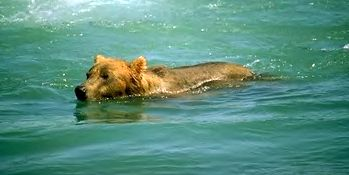
\includegraphics[width=\textwidth]{../../data/BearInWater.jpg}
				\caption{源图片}
			\end{subfigure}
			\begin{subfigure}[htbp]{0.36\textwidth}
				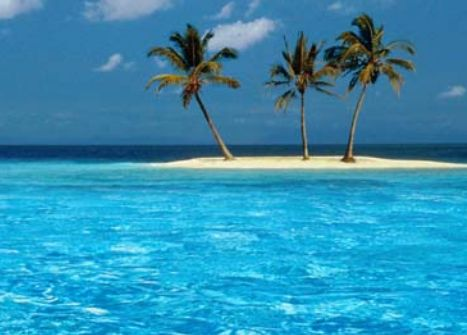
\includegraphics[width=\textwidth]{../../data/NewBackGround.jpg}
				\caption{背景图片}
			\end{subfigure}
			\caption{熊与水背景}
		\end{figure}

		\begin{figure}[ht]
			\centering
			\begin{subfigure}[htbp]{0.36\textwidth}
				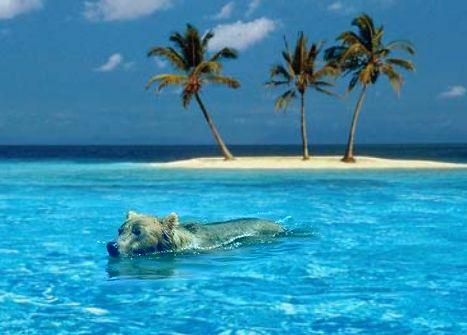
\includegraphics[width=\textwidth]{../../result/result_00.jpg}
				\caption{普通融合}
			\end{subfigure}
			\begin{subfigure}[htbp]{0.36\textwidth}
				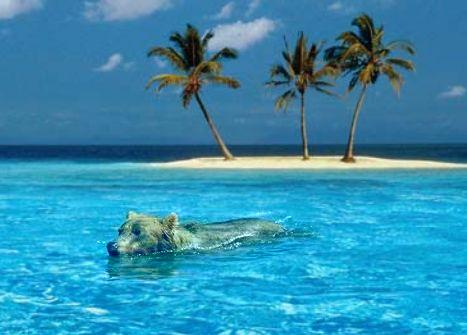
\includegraphics[width=\textwidth]{../../result/result_01.jpg}
				\caption{混合梯度融合}
			\end{subfigure}
			\caption{融合结果对比 1}
		\end{figure}

		\begin{figure}[ht]
			\centering
			\begin{subfigure}[htbp]{0.36\textwidth}
				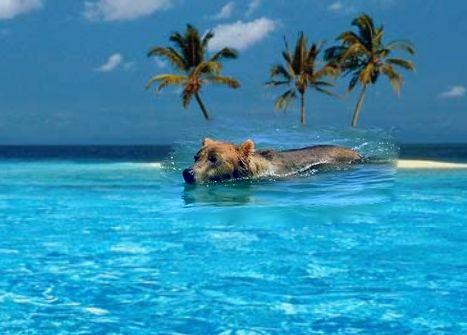
\includegraphics[width=\textwidth]{../../result/result_10.jpg}
				\caption{普通融合}
			\end{subfigure}
			\begin{subfigure}[htbp]{0.36\textwidth}
				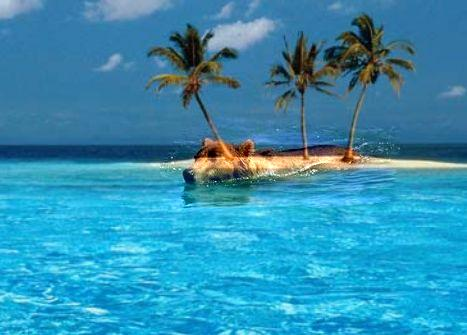
\includegraphics[width=\textwidth]{../../result/result_11.jpg}
				\caption{混合梯度融合}
			\end{subfigure}
			\caption{融合结果对比 2}
		\end{figure}

		\begin{figure}[ht]
			\centering
			\begin{subfigure}[htbp]{0.45\textwidth}
				
\includegraphics[width=\textwidth]{../../data/test_src.jpg}
				\caption{源图片}
			\end{subfigure}
			\begin{subfigure}[htbp]{0.45\textwidth}
				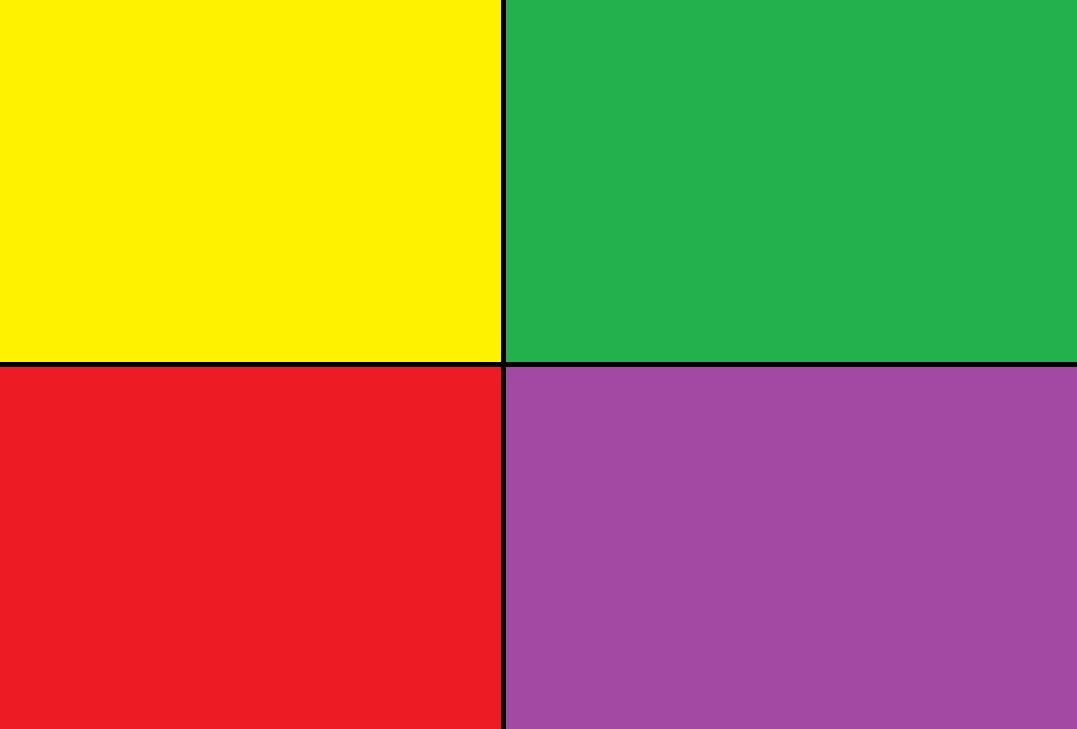
\includegraphics[width=\textwidth]{../../data/test_target.jpg}
				\caption{背景图片}
			\end{subfigure}
			\caption{色块}
		\end{figure}

		\begin{figure}[ht]
			\centering
			\begin{subfigure}[htbp]{0.45\textwidth}
				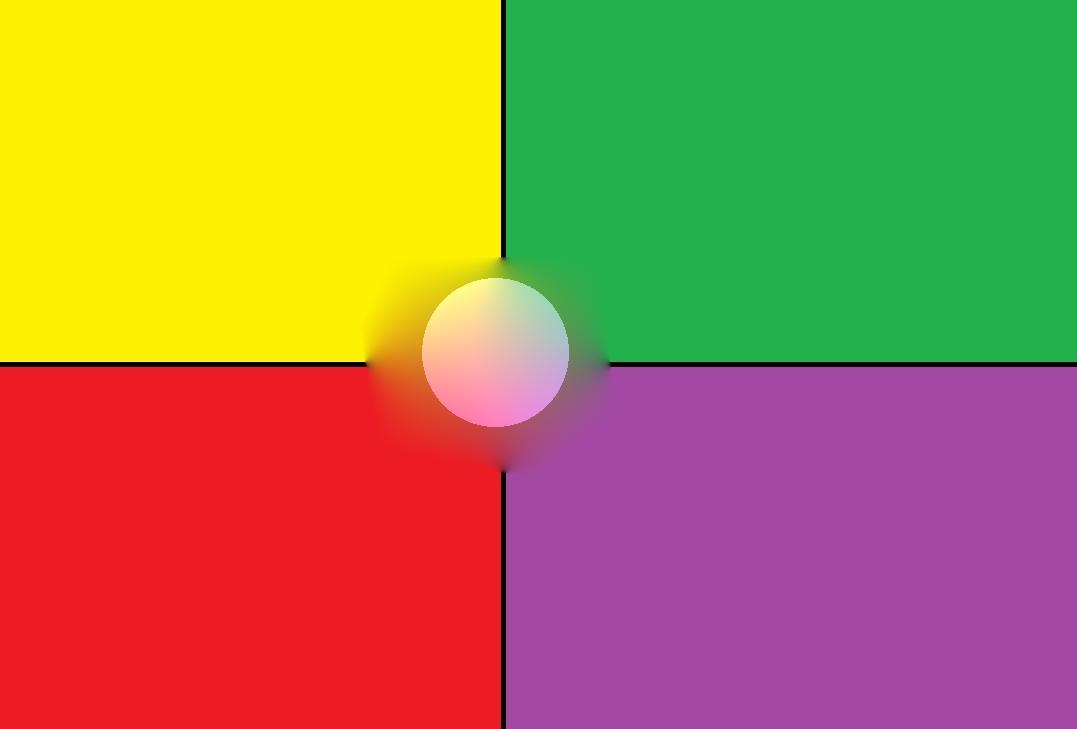
\includegraphics[width=\textwidth]{../../result/result_20.jpg}
				\caption{普通融合}
			\end{subfigure}
			\begin{subfigure}[htbp]{0.45\textwidth}
				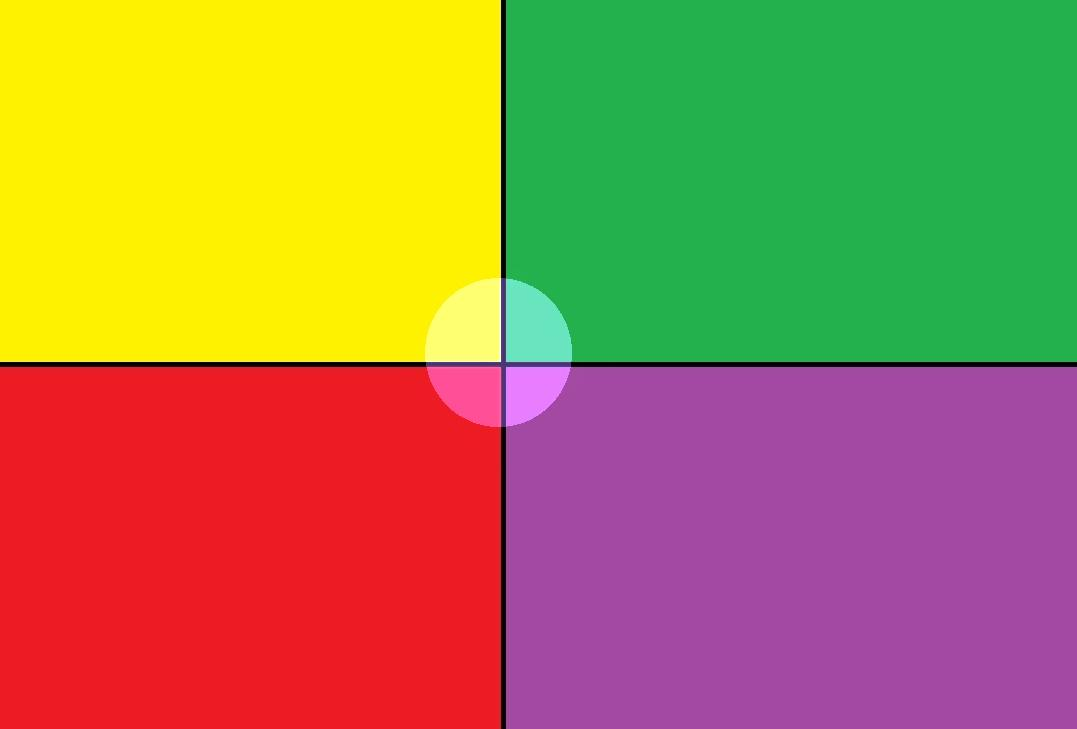
\includegraphics[width=\textwidth]{../../result/result_21.jpg}
				\caption{混合梯度融合}
			\end{subfigure}
			\caption{融合结果对比}
		\end{figure}

		\begin{figure}[ht]
			\centering
			\begin{subfigure}[htbp]{0.45\textwidth}
				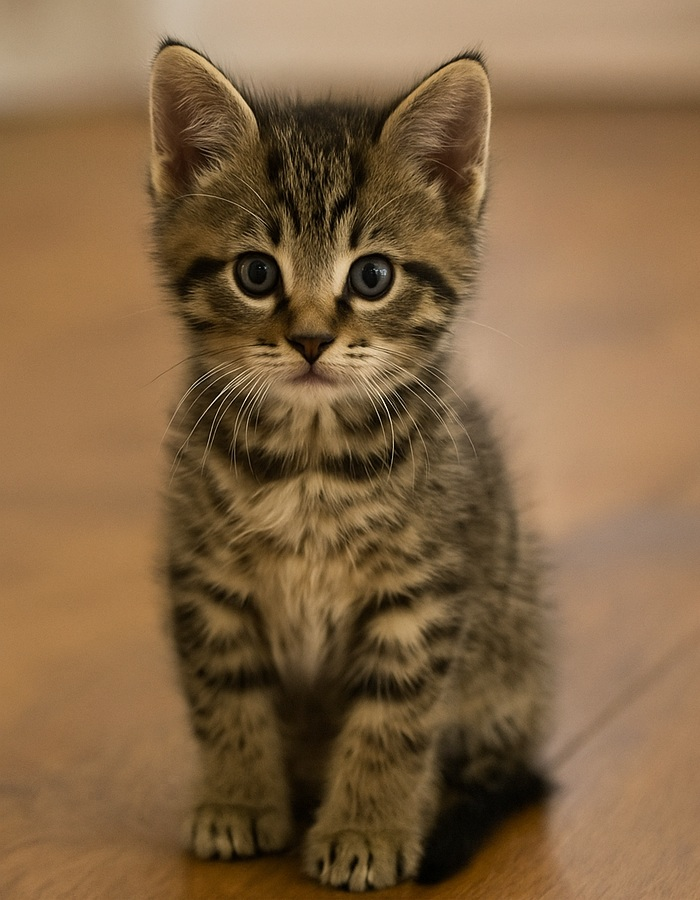
\includegraphics[width=\textwidth]{../../data/cat.png}
				\caption{源图片}
			\end{subfigure}
			\begin{subfigure}[htbp]{0.45\textwidth}
				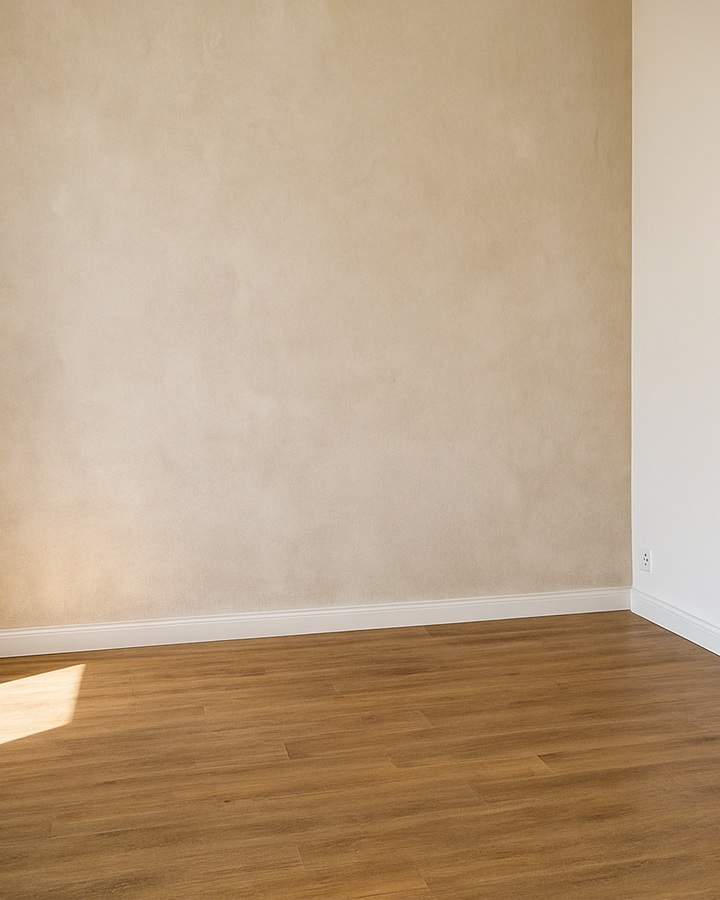
\includegraphics[width=\textwidth]{../../data/room.png}
				\caption{背景图片}
			\end{subfigure}
			\caption{小猫与空房间}
		\end{figure}

		\begin{figure}[ht]
			\centering
			\begin{subfigure}[htbp]{0.45\textwidth}
				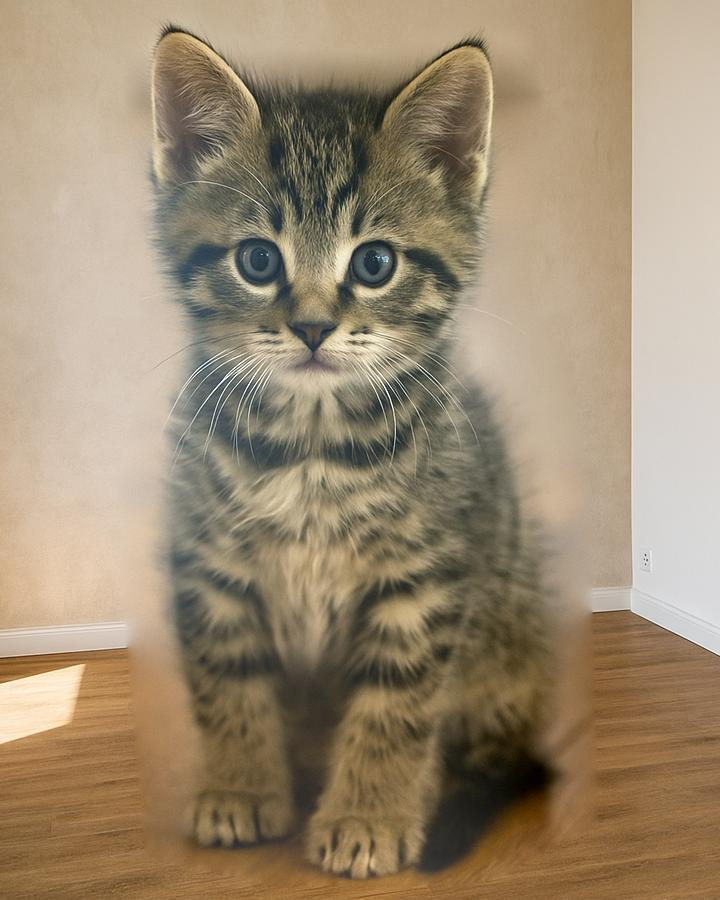
\includegraphics[width=\textwidth]{../../result/result_30.jpg}
				\caption{普通融合}
			\end{subfigure}
			\begin{subfigure}[htbp]{0.45\textwidth}
				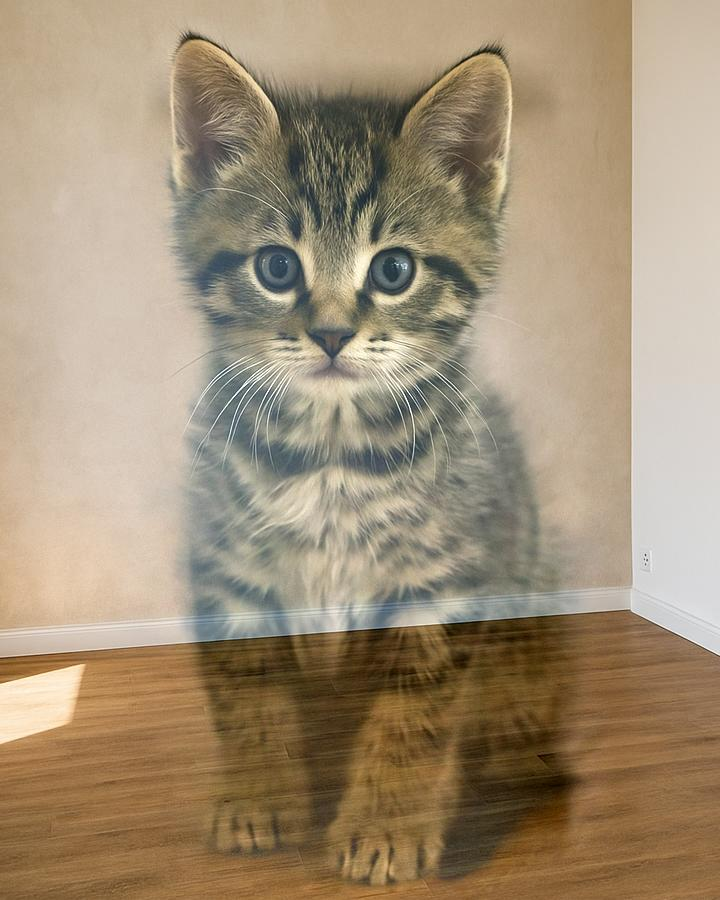
\includegraphics[width=\textwidth]{../../result/result_31.jpg}
				\caption{混合梯度融合}
			\end{subfigure}
			\caption{融合结果对比}
		\end{figure}

\end{document}
